\documentclass{article}

\usepackage{amsfonts}
\usepackage{tikz}
\usetikzlibrary{shapes, backgrounds}

\title{Sets}

\def\firstcircle{(0.75,0) circle (1)}
\def\specs{(0.75, 1) node [text=black, above left] {Wear spectacles}}
\def\secondcircle{(1.75, 0) circle (1)}
\def\name{(1.75, -1) node [text=black, below right] {Name starts with `P'}}
\def\rectangle{(-2, -2) rectangle (4.5, 2) (1, 2) node [text=black, above] {classmates}}
\def\N{\mathbb{N}}
\setlength{\parindent}{0cm}

\begin{document}
\maketitle

\begin{minipage}{\textwidth}
Let us begin by talking about your classmates.

\vspace{1em}

\begin{tikzpicture}[fill=gray]
	\draw \rectangle;
\end{tikzpicture}
\end{minipage}

\vspace{1em}

\begin{minipage}{0.49\textwidth}%
Now, among your classmates, there are some students who wear spectacles.

\vspace{1em}

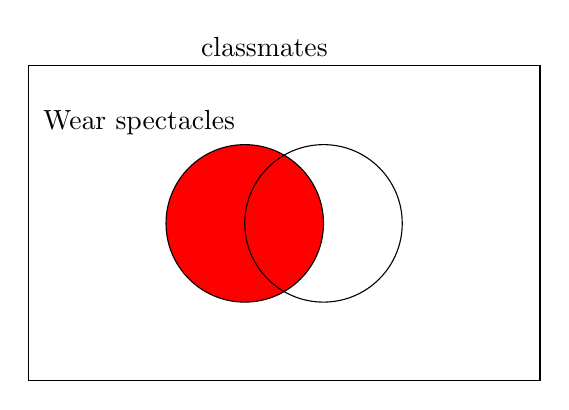
\begin{tikzpicture}[fill=red]
%	\clip(1, 0) circle(1);
%	\fill (0.5, 0) circle(1);
%	\draw (-2, -2) rectangle(4, 2) (1, 2) node [text=black, above] {classmates};
%	\draw (0.5, 0) circle(1) (0.5, 1) node [text=black, above left] {Wear spectacles};
%	\draw (1.5, 0) circle(1);

	\fill \firstcircle;
	\draw \firstcircle \specs;
	\draw \secondcircle;
	\draw \rectangle;
\end{tikzpicture}
\end{minipage}%
\hspace{1cm}%
%
\begin{minipage}{0.49\textwidth}

And there are some whose names start with `P'.

\vspace{1em}

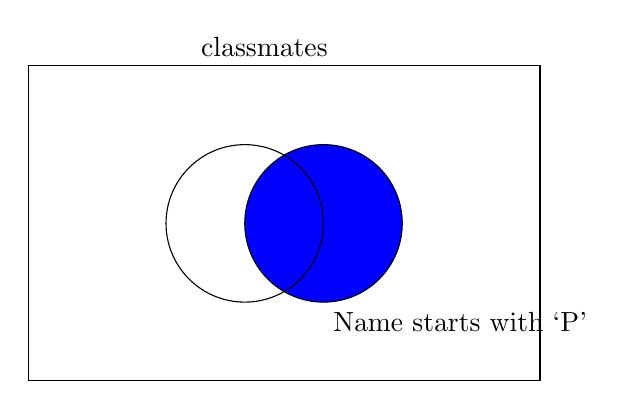
\begin{tikzpicture}[fill=blue]
%	\clip (0, 0) circle(1);
%	\fill (1.5, 0) circle(1);
%
%	\draw (-2, -2) rectangle(4, 2) (1, 2) node [text=black, above] {classmates};
%	\draw (0.5, 0) circle(1) (0, 1);
%	\draw (1.5, 0) circle(1) (1.5, -1) node [text=black, below right] {Name starts with `P'};

	\fill \secondcircle;
	\draw \firstcircle;
	\draw \secondcircle \name;
	\draw \rectangle;
\end{tikzpicture}

\end{minipage}

\vspace{1em}

\begin{minipage}{\textwidth}
Then there are some who wear spectacles \emph{and} their name starts with `P'.

\vspace{1em}

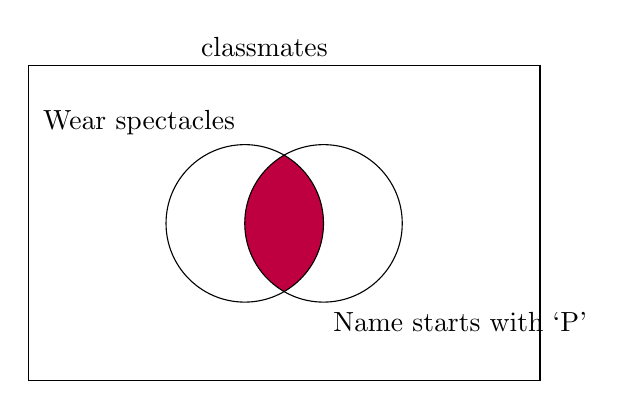
\begin{tikzpicture}[fill=purple]
	\begin{scope}[even odd rule, overlay]
	\clip \firstcircle;
	\clip \secondcircle;
	\fill \firstcircle;
	\fill \secondcircle;
	\end{scope}

	\draw \rectangle;
	\draw \firstcircle \specs;
	\draw \secondcircle \name;
\end{tikzpicture}

\end{minipage}

\vspace{1em}

You can even think about the classmates who either wear spectacles \emph{or} have
names starting with `P', \emph{or} both.

\vspace{1em}

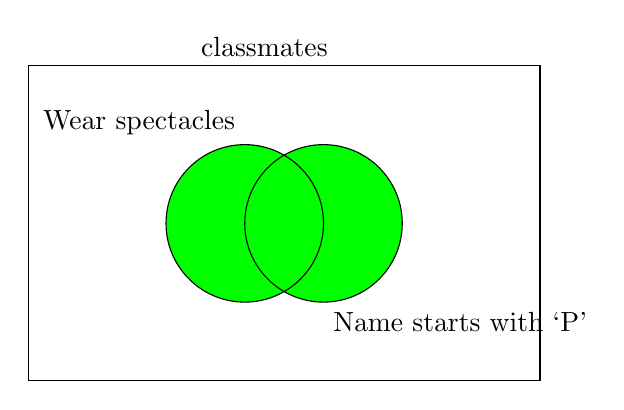
\begin{tikzpicture}[fill=green]
	\begin{scope}[even odd rule, overlay]
	\fill \firstcircle;
	\fill \secondcircle;
	\end{scope}

	\draw \rectangle;
	\draw \firstcircle \specs;
	\draw \secondcircle \name;
\end{tikzpicture}

\vspace{1em}

If you have enough classmates, there might even by some whose names start with `P', and
end with `H'.

\vspace{1em}

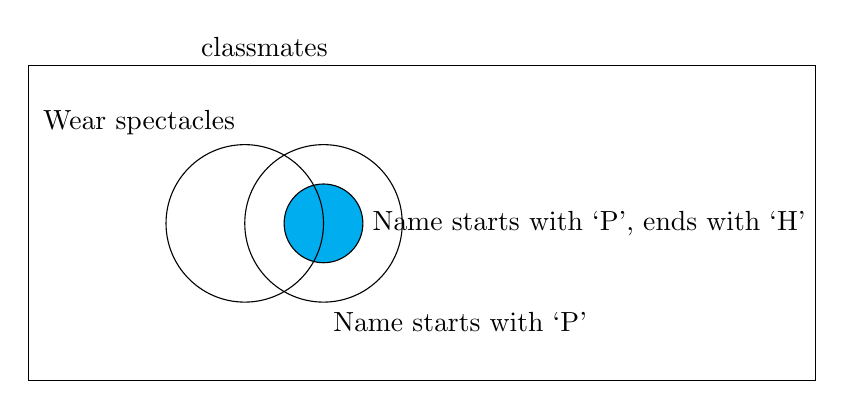
\begin{tikzpicture}[fill=cyan]
	\fill (1.75, 0) circle(0.5);

	\draw (-2, -2) rectangle(8, 2) (1, 2) node [text=black, above] {classmates};
	\draw \firstcircle \specs;
	\draw \secondcircle \name;
	\draw (1.75, 0) circle(0.5) (2.25, 0) node [text=black, right] {Name starts with `P', ends with `H'};
\end{tikzpicture}

\vspace{1em}

Finally, we might be interested in all of your classmates whose names \emph{don't}
start with `P'.

\vspace{1em}

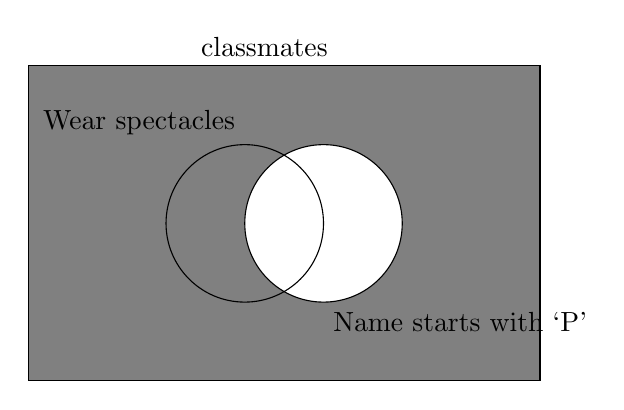
\begin{tikzpicture}[fill=gray]
%	\begin{scope}[even odd rule, overlay]
%		\clip (-2, -2) rectangle(4.5, 2);
%		\clip \secondcircle;
%		\fill (-2, -2) rectangle(4.5, 2);
%	\end{scope}
	\fill (-2, -2) rectangle(4.5, 2);
	\fill [white] \secondcircle;
	\draw \firstcircle \specs;
	\draw \secondcircle \name;
	\draw \rectangle;
\end{tikzpicture}

\vspace{1em}

Phew, that was a lot of thinking, but how is this related to \emph{Sets}?.

\section{What is a Set?}

%Note: In this section, we will be introducing a lot of new words.
%You do not need to memorize what they are, if you forget something,
%just come back to where we talked about it first.

%\vspace{1em}

Actually, in all of the previous examples, you were working with sets. \\
All of your classmates who wear spectacles? A set. \\ 
All of your classmates whose names start with `P'? Also a set.

\vspace{1em}

%We even did most of the set \emph{operations}.
%
%Remember the part where you thought about your classmates who wear spectacles, \emph{and} have names
%starting with `P'? That is called the \emph{intersection} operation.
%
%And the part where you thought about your classmates who wear spectacles, \emph{or} have names starting
%with `P', \emph{or} both? That is called the \emph{union} operation.
%
%\vspace{1em}

In general, 
we will think of a set as a collection of objects.
What kind of objects? Numbers, chairs, classmates, anything.

Anything?

Yes \footnote{for the purpose of this write-up}, anything.
We can use the ideas here to talk about sets of potatoes, sets
of integers, sets of cars, whatever we like.

So, let us now begin to work with sets (yay!)

\subsection{Universe}
The first thing to do, is to pick a \emph{universe}
(the giant rectangular box surrounding everything)
to work in.
In the first example, our universe was all of your classmates.

Very often, we will be working with a universe of natural numbers.
In this universe, we don't talk about fractions, or negative integers
very much, just like in the universe of your classmates we don't talk about
your teachers, or your friends from around your home.

Why do we pick a universe?
It is very annoying to be talking about numbers, and all of a sudden a potato
comes into the discussion out of nowhere.
So we pick a universe so that we know what kind of objects we are talking about,
and to avoid unnecessary confusion.

\subsection{Writing sets}
After we've picked a universe, we have several ways of writing sets.
Most of the time, we ``let'' a capital letter denote the set, 
so that it is easy to refer to it.

\vspace{1em}

So one way to define a set is to loosely describe it.
For example, one can say
``Let $C =$ the set of all of your classmates''.
Which is perfectly acceptable, we can think about this set
very naturally in the universe of your classmates.

Another example is saying something like
``Let $\N = $ the set of all natural numbers''.
Which is also acceptable in the universe of natural numbers.

\vspace{1em}

Another way is to write out all of the set's elements.
For example, we can have a small set of your classmates, like
$D = \left\{\texttt{``Pappu''}, \texttt{``Suresh''}, \texttt{``Asha''}\right\}$
\footnote{maybe you would like to change these names},
which is a set in the universe of your classmates.

Another example, is the set $J = \left\{1, 2, 3\right\}$, in the universe of natural numbers.

Note how we are writing these sets. We first write a $\{$, followed by all
of the \emph{elements} of the set (separated by commas), followed by $\}$.

There are a few additional rules to writing sets this way.
\begin{itemize}
	\item The order you write the elements in does not matter.
		So the set $\left\{1, 2, 3, 4, 5\right\}$ is the same
		as the set $\left\{3, 1, 2, 5, 4\right\}$.
	\item It doesn't matter how many times you repeat an element.
		So the set $\left\{1, 1, 2, 3, 3, 3, 4, 5\right\}$ is the
		same as the set $\left\{1, 2, 3, 4, 5\right\}$.
\end{itemize}

\subsection{The empty set}
Often, we will deal with a set which is actually empty, that is, it has
no elements. We use $\{\}$ to denote the empty set.

An example of an empty set is the set of your classmates who are taller
than 15 feet.

\subsection{Intersections and Unions}
In the initial example, we were working with two sets of your classmates.
Let $P = $ the set of your classmates whose names start with `P', and let
$S = $ the set of your classmates who wear spectacles.

Then the classmates who belong to both of these sets (that is, those whose names start
with `P' and they wear spectacles), belong to the \emph{intersection} of 
these sets, which is also another set.
The symbol $\cap$ is used to denote intersection.
So $P \cap S$ is the intersection of $P$ and $S$, which we described above.

Further, the classmates who belong to either (or both) of these sets are all part
of the \emph{union} of the sets (which is again, also a set).
The symbol $\cup$ is used to denote union.
So $P \cup S$ is the union of $P$ and $S$, as described above.

\subsubsection{Exercises}
\begin{itemize}
	\item If $E$ is the set of all even natural numbers, and $O$ is the set of
	all odd natural numbers, then what is $E \cup O$.
	\item With the same definitions of $E$ and $O$, what is $E \cap O$?
\end{itemize}

\subsection{Subsets and membership}
Remember how we talked about the set of your classmates whose names start
with `P' and end with `H'? Let us denote this set by $H$.
Then we notice something interesting. If there is any student who belongs
to this set $H$, they also automatically belong to $P$ (the set of classmates
whose name begins with `P').
So every element of $H$ is also an element of $P$.
This is also apparent from the diagram we saw earlier (the circle for $H$ is contained
within the circle for $P$).

We write this as $H$ is a \emph{subset} of $P$, or $H \subset P$.

For another example, let's look at the set of even natural numbers, $E$.
Every element of $E$ is also an element of $\N$, so
$E$ is a subset of $\N$, or $E \subset N$.

By the definition above, is every set a subset of itself?
Is the empty set a subset of every set?

Very often when we are talking about sets, we will make statements
about individual members of the set, like 
$1$ is an element of $\N$. For this, we have the symbol $\in$,
which is to be read as ``is an element of''.
So we can use it in statements like $1 \in \N$, which translates to
$1$ is an element of $\N$.

\subsubsection{Exercises}
\begin{itemize}
	\item List all of the subsets of $\left\{ 1, 2, 3 \right\}$
		(there are 8 subsets).
	\item Is $\frac 12 \in \N$ true?
\end{itemize}

\vspace{1em}

\subsection{Complements}
Sometimes, we will be interested in the set of everything that is \emph{not} in 
a particular set.

For example, we might be interested in all of your classmates whose names do not
start with `P'.
Note that this would be exactly those classmates who do not belong to $P$.
We use the symbol $\overline{P}$ to denote this.

In general, the $\overline{A}$ of some set $A$ is the set which contains everything
in the universe which does not belong to $A$.

So, for example, in the universe of natural numbers, $\overline{E}$ is equal to $O$.

\subsubsection{Exercises}
\begin{itemize}
	\item Describe the set $\overline{S}$, where $S$ is the set of your classmates
	who wear spectacles.
\end{itemize}

%What if we want to talk about a somewhat large set? 
%Say, for example, the set which consists of all the natural numbers smaller than $100$.
%
%We could write out the set like $\{1, 2, 3, 4, \dots$ and so on up until $100$.
%This is of course, rather inconvenient.
%
%So we use \emph{set-builder} notation.
%In this way of defining sets, instead of listing out each element, we
%provide a few conditions on what can be a member of the set.
%
%Working with the example above, the two conditions we want on every element of
%the set are:
%\begin{itemize}
%	\item Should be a natural number.
%	\item Should be smaller than or equal to $100$.
%\end{itemize}
%
%The corresponding definition is
%$\left\{x \mid x \texttt{ is a natural number}, x \leq 100\right\}$.
%
%This is read as ``the set which contains all such $x$, which are natural numbers
%\emph{and} $\leq 100$''.
%
%Essentially, to the right of the vertical line ``$\mid$'' we write the conditions
%we require some value to obey, and on the left of the line, we write what we wish to
%do with every such value.
%
%In the example above, we are simply adding every value which obeys the conditions
%to the set as is.
%In general, however, we can apply any mathematical operation to the value before adding
%it to the set.
%
%So, for example, we can construct a set
%$\left\{x^2 \mid x \texttt{ is a natural number}, x \leq 100\right\}$.
%This is almost the same set as before, except we are squaring each number,
%so instead of constructing the set $\{1, 2, 3, \dots$ upto $100$, this will
%construct $\{1^2, 2^2, 3^2, 4^2, \dots$ upto $100^2$.

\end{document}
